\section{Resultados e Discussão}
\label{sec:resultados}

Todas as métricas desta seção foram calculadas exclusivamente sobre o conjunto de teste de cada edição ($n = 10.000$), e as tabelas e figuras são geradas automaticamente a partir dos arquivos Parquet do pipeline.

\subsection{Desempenho do Modelo-Alvo}
\label{sec:res_desempenho}

Nas três edições, a busca em grade selecionou a mesma configuração (100 árvores, profundidade máxima 3 e taxa de aprendizado 0,1), e o desempenho manteve-se estável: acurácia entre 0,6822 e 0,6842 e AUC-ROC entre 0,7475 e 0,7511 (Tabela~\ref{tab:desempenho}). Os três hiperparâmetros situam-se nos limites da grade, o que indica que uma grade mais ampla poderia produzir ganhos marginais, não perseguidos porque o modelo é o \textbf{objeto} da auditoria, e não o produto do trabalho. O F1 (entre 0,674 e 0,677) é inferior, mas da mesma ordem de grandeza, ao de \cite{luz2025uso} (0,758), que, porém, empregam mais variáveis e tomam como classe positiva o desempenho \textbf{abaixo} da média. Um modelo com AUC-ROC próxima de 0,75 seria considerado razoável em muitas aplicações, e é justamente esse tipo de modelo, aparentemente aceitável, que a ferramenta deve examinar.

% ARQUIVO GERADO AUTOMATICAMENTE por article/scripts/gerar_resultados.py
% Fonte: data/outputs/*.parquet — NÃO EDITAR À MÃO.
\begin{table}[htbp]
\centering
\caption{Desempenho do modelo-alvo (XGBoost) no conjunto de teste}
\label{tab:desempenho}
\resizebox{\textwidth}{!}{%
\begin{tabular}{lccccccc}
\toprule
\textbf{Edição} & \textbf{Acurácia} & \textbf{Precisão} & \textbf{Recall} & \textbf{F1} & \textbf{AUC-ROC} & \textbf{n\_est. / prof. / taxa} & \textbf{$n_{\text{teste}}$} \\
\midrule
2019 & 0,6842 & 0,7000 & 0,6490 & 0,6736 & 0,7511 & 100 / 3 / 0,10 & 10.000 \\
2020 & 0,6825 & 0,6926 & 0,6584 & 0,6751 & 0,7475 & 100 / 3 / 0,10 & 10.000 \\
2021 & 0,6822 & 0,6868 & 0,6673 & 0,6769 & 0,7480 & 100 / 3 / 0,10 & 10.000 \\
\bottomrule
\end{tabular}}
\fonte{\elaboradopor{} a partir de \texttt{model\_metrics\_\{ano\}.parquet}.}
\end{table}


\subsection{Equidade por Raça/Cor}
\label{sec:res_raca}

Em todas as edições, o grupo de referência é o de candidatos brancos, e \textbf{todos os grupos não brancos apresentam DI inferior a 0,8} (Tabela~\ref{tab:di_raca}). Os grupos Preta e Parda, que juntos representam mais da metade dos candidatos, apresentam as disparidades mais consistentes e com tendência de agravamento: o DI do grupo Preta passa de 0,426 em 2019 para 0,365 em 2020 e 0,337 em 2021, e o do grupo Parda, de 0,495 para 0,462 e 0,423. Em 2021, um candidato preto tinha cerca de um terço da probabilidade de um candidato branco de ser classificado acima da mediana.

% ARQUIVO GERADO AUTOMATICAMENTE por article/scripts/gerar_resultados.py
% Fonte: data/outputs/*.parquet — NÃO EDITAR À MÃO.
\begin{table}[htbp]
\centering
\caption{Impacto Disparate e Igualdade de Oportunidades por raça/cor no conjunto de teste, com intervalos de confiança de 95\%}
\label{tab:di_raca}
\resizebox{\textwidth}{!}{%
\begin{tabular}{lccccccc}
\toprule
\textbf{Grupo} & \textbf{$n$} & \textbf{$n$ ($Y=1$)} & \textbf{DI} & \textbf{IC95\% DI} & \textbf{TPR} & \textbf{IC95\% TPR} & \textbf{DI $<$ 0,8} \\
\midrule
\multicolumn{8}{l}{\textbf{ENEM 2019}} \\
\quad Branca (ref.) & 3.723 & 2.341 & 1,000 & -- & 0,801 & [0,784; 0,817] & Não \\
\quad Preta & 1.219 & 488 & 0,426 & [0,387; 0,465] & 0,469 & [0,424; 0,515] & \textbf{Sim} \\
\quad Parda & 4.581 & 1.954 & 0,495 & [0,472; 0,518] & 0,521 & [0,498; 0,542] & \textbf{Sim} \\
\quad Amarela & 225 & 106 & 0,609 & [0,517; 0,705] & 0,623 & [0,531; 0,710] & \textbf{Sim} \\
\quad Indígena & 52 & 19 & 0,252 & [0,115; 0,414] & 0,316 & [0,125; 0,545] & \textbf{Sim} \\
\quad Não declarada & 200 & 112 & 0,620 & [0,522; 0,720] & 0,580 & [0,491; 0,675] & \textbf{Sim} \\
\midrule
\multicolumn{8}{l}{\textbf{ENEM 2020}} \\
\quad Branca (ref.) & 3.793 & 2.386 & 1,000 & -- & 0,842 & [0,827; 0,856] & Não \\
\quad Preta & 1.227 & 483 & 0,365 & [0,331; 0,400] & 0,418 & [0,373; 0,460] & \textbf{Sim} \\
\quad Parda & 4.505 & 1.909 & 0,462 & [0,441; 0,484] & 0,505 & [0,483; 0,528] & \textbf{Sim} \\
\quad Amarela & 230 & 117 & 0,498 & [0,417; 0,587] & 0,496 & [0,406; 0,589] & \textbf{Sim} \\
\quad Indígena & 49 & 12 & 0,169 & [0,048; 0,310] & 0,167 & [0,000; 0,429] & \textbf{Sim} \\
\quad Não declarada & 196 & 102 & 0,633 & [0,539; 0,735] & 0,627 & [0,533; 0,726] & \textbf{Sim} \\
\midrule
\multicolumn{8}{l}{\textbf{ENEM 2021}} \\
\quad Branca (ref.) & 4.427 & 2.730 & 1,000 & -- & 0,830 & [0,816; 0,844] & Não \\
\quad Preta & 1.104 & 405 & 0,337 & [0,302; 0,373] & 0,343 & [0,298; 0,390] & \textbf{Sim} \\
\quad Parda & 4.022 & 1.643 & 0,423 & [0,401; 0,444] & 0,477 & [0,453; 0,501] & \textbf{Sim} \\
\quad Amarela & 211 & 109 & 0,663 & [0,570; 0,759] & 0,706 & [0,617; 0,792] & \textbf{Sim} \\
\quad Indígena & 47 & 9 & 0,417 & [0,231; 0,613] & 0,778 & [0,429; 1,000] & \textbf{Sim} \\
\quad Não declarada & 189 & 93 & 0,629 & [0,530; 0,731] & 0,602 & [0,500; 0,703] & \textbf{Sim} \\
\bottomrule
\end{tabular}}
\fonte{\elaboradopor{} a partir de \texttt{fairness\_metrics\_\{ano\}.parquet}. Grupo de referência: maior taxa de seleção. IC95\%: percentis 2,5 e 97,5 de 2.000 reamostragens \textit{bootstrap} do conjunto de teste, com o modelo fixo. A FPR por grupo é apresentada na Figura~\ref{fig:tpr_fpr}.}
\end{table}


O \textbf{alerta é estatisticamente robusto para todos os grupos não brancos}, inclusive o Indígena: o limite superior do IC95\% do DI não ultrapassa 0,759 em nenhum caso, e em ao menos 99,5\% das reamostragens o DI permaneceu abaixo de 0,8. A tendência de agravamento dos grupos Preta e Parda também é sustentada, pois os intervalos de 2019 e 2021 não se sobrepõem. Já o grupo Indígena conta com apenas 47 a 52 candidatos no teste, e \textbf{suas estimativas de TPR não são conclusivas}: com 19, 12 e 9 rótulos positivos, os intervalos são muito amplos ([0,000; 0,429] em 2020 e [0,429; 1,000] em 2021), e a TPR de 0,778 em 2021 não deve ser lida como evidência de igualdade de oportunidades; a variação abrupta do DI indígena em 2021 (0,417) é compatível com flutuação amostral.

O modelo também \textbf{erra de forma assimétrica} (Figura~\ref{fig:tpr_fpr}). Entre os candidatos com NMG igual ou superior à mediana, reconhece entre 80,1\% e 84,2\% dos brancos, mas apenas 46,9\%, 41,8\% e 34,3\% dos pretos em 2019, 2020 e 2021, e entre 47,7\% e 52,1\% dos pardos. Simetricamente, a FPR de candidatos brancos (0,492 a 0,530) é cerca de três vezes a de pretos (0,165 a 0,182). O modelo concede mais classificações acima da mediana indevidas ao grupo privilegiado e nega mais classificações merecidas aos grupos protegidos, violando os critérios de \textit{Equal Opportunity} e \textit{Equalized Odds}.

\begin{figure}[htbp]
\centering
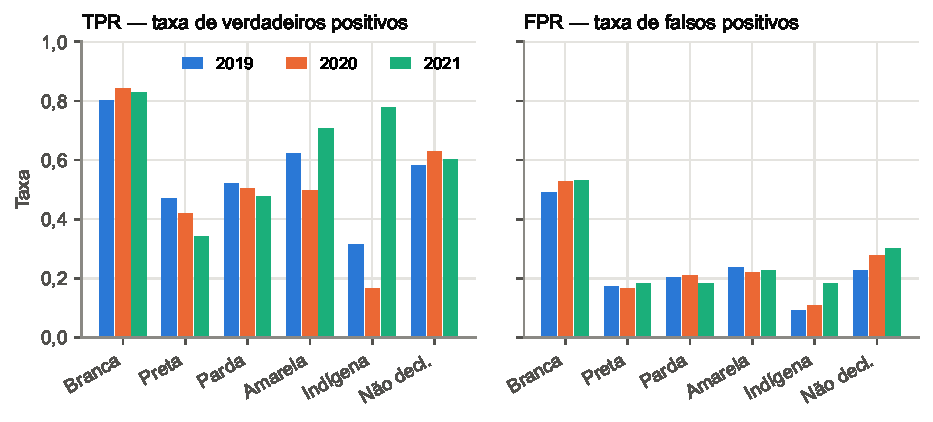
\includegraphics[width=0.85\textwidth]{../article/figuras/resultados/fig_tpr_fpr_raca.pdf}
\caption{Taxas de verdadeiros positivos (TPR) e de falsos positivos (FPR) por raça/cor}
\label{fig:tpr_fpr}
\fonte{Elaborado pelos autores a partir de \texttt{fairness\_metrics\_\{ano\}.parquet}.}
\end{figure}

\subsection{Equidade por Renda Familiar}
\label{sec:res_renda}

A renda familiar produz o gradiente mais acentuado (Tabela~\ref{tab:di_renda}). Nas três edições, \textbf{as faixas A a E (até 2,5 salários mínimos) violam a regra dos quatro quintos}, e as faixas A e B têm DI entre 0,044 e 0,074: o modelo praticamente nunca classifica esses candidatos acima da mediana. Na faixa B, a TPR é de apenas 0,077, 0,126 e 0,115 em 2019, 2020 e 2021, ou seja, quase nove em cada dez candidatos de baixa renda que superaram a mediana são classificados incorretamente. A fronteira do alerta situa-se entre as faixas E e F. Na faixa E, o DI fica abaixo de 0,8 em pelo menos 98\% das reamostragens nas três edições; já a faixa F em 2021 ($\mathrm{DI} = 0{,}803$, IC95\% [0,774; 0,832]) encontra-se \textbf{sobre o limiar}, com DI abaixo de 0,8 em 41,2\% das reamostragens, e a ausência de alerta não deve ser lida como conformidade. Como várias faixas superiores empatam com taxas de seleção próximas de 100\%, a referência varia entre as edições (L, J e L), sem impacto relevante sobre as faixas inferiores; e, como os limites das faixas são expressos em salários mínimos de cada ano, a comparação entre edições é relativa.

% ARQUIVO GERADO AUTOMATICAMENTE por article/scripts/gerar_resultados.py
% Fonte: data/outputs/*.parquet — NÃO EDITAR À MÃO.
\begin{table}[htbp]
\centering
\caption{Impacto Disparate e TPR por faixa de renda familiar (Q006) no conjunto de teste}
\label{tab:di_renda}
\begin{tabular}{llcccccc}
\toprule
 & & \multicolumn{3}{c}{\textbf{DI}} & \multicolumn{3}{c}{\textbf{TPR}} \\
\cmidrule(lr){3-5}\cmidrule(lr){6-8}
\textbf{Faixa} & \textbf{Renda mensal} & 2019 & 2020 & 2021 & 2019 & 2020 & 2021 \\
\midrule
A & Nenhuma renda & \textbf{0,070} & \textbf{0,072} & \textbf{0,044} & 0,190 & 0,181 & 0,108 \\
B & Até 1 SM & \textbf{0,047} & \textbf{0,074} & \textbf{0,053} & 0,077 & 0,126 & 0,115 \\
C & 1 a 1,5 SM & \textbf{0,209} & \textbf{0,356} & \textbf{0,207} & 0,284 & 0,447 & 0,290 \\
D & 1,5 a 2 SM & \textbf{0,662} & \textbf{0,569} & \textbf{0,481} & 0,736 & 0,664 & 0,575 \\
E & 2 a 2,5 SM & \textbf{0,771} & \textbf{0,764} & \textbf{0,723} & 0,858 & 0,827 & 0,767 \\
F & 2,5 a 3 SM & 0,848 & 0,855 & 0,803 & 0,884 & 0,883 & 0,869 \\
G & 3 a 4 SM & 0,897 & 0,947 & 0,883 & 0,921 & 0,961 & 0,911 \\
H & 4 a 5 SM & 0,976 & 0,982 & 0,938 & 0,983 & 0,989 & 0,961 \\
I & 5 a 6 SM & 0,968 & 0,983 & 0,974 & 0,981 & 0,984 & 0,973 \\
J & 6 a 7 SM & 0,995 & 1,000 & 0,990 & 0,994 & 1,000 & 0,987 \\
K & 7 a 8 SM & 0,986 & 0,992 & 0,981 & 1,000 & 1,000 & 0,991 \\
L & 8 a 9 SM & 1,000 & 1,000 & 1,000 & 1,000 & 1,000 & 1,000 \\
M & 9 a 10 SM & 0,989 & 1,000 & 0,986 & 0,987 & 1,000 & 0,988 \\
N & 10 a 12 SM & 1,000 & 1,000 & 0,993 & 1,000 & 1,000 & 0,991 \\
O & 12 a 15 SM & 0,990 & 1,000 & 0,992 & 1,000 & 1,000 & 0,991 \\
P & 15 a 20 SM & 1,000 & 0,991 & 0,985 & 1,000 & 1,000 & 0,991 \\
Q & Acima de 20 SM & 1,000 & 1,000 & 1,000 & 1,000 & 1,000 & 1,000 \\
\bottomrule
\end{tabular}
\fonte{\elaboradopor{} a partir de \texttt{fairness\_metrics\_\{ano\}.parquet}. SM = salário mínimo vigente no ano. Em negrito: DI $<$ 0,8. Faixa de referência (maior taxa de seleção) --- 2019: L, 2020: J, 2021: L.}
\end{table}


\subsection{Amplificação do Viés pelo Modelo}
\label{sec:res_amplificacao}

A Tabela~\ref{tab:amplificacao} compara o DI dos rótulos reais com o das predições (Equação~\ref{eq:amplificacao}). Em 14 das 15 combinações de grupo e edição, o DI das predições é inferior ao dos rótulos, com reduções entre 0,140 e 0,329, e em 13 delas o IC95\% de $\Delta_g$ fica inteiramente abaixo de zero. As duas exceções são do grupo Indígena: em 2020, a estimativa é negativa ($-0{,}220$), mas o intervalo inclui zero; em 2021, $\Delta_g = +0{,}106$, com intervalo [$-0{,}070$; 0,296]. Para esse grupo, a amplificação só é sustentada em 2019, e nem a amplificação de 2020 nem a atenuação de 2021 podem ser distinguidas de zero.

% ARQUIVO GERADO AUTOMATICAMENTE por article/scripts/gerar_resultados.py
% Fonte: data/outputs/*.parquet — NÃO EDITAR À MÃO.
\begin{table}[htbp]
\centering
\caption{Impacto Disparate dos rótulos reais ($y$) versus das predições ($\hat{y}$) por raça/cor, com intervalos de confiança de 95\%}
\label{tab:amplificacao}
\begin{tabular}{lccccc}
\toprule
\textbf{Grupo} & $\mathrm{DI}_y$ & \textbf{IC95\%} $\mathrm{DI}_y$ & $\mathrm{DI}_{\hat{y}}$ & $\Delta$ & \textbf{IC95\%} $\Delta$ \\
\midrule
\multicolumn{6}{l}{\textbf{ENEM 2019}} \\
\quad Preta & 0,637 & [0,590; 0,684] & 0,426 & \textbf{−0,211} & [−0,264; −0,160] \\
\quad Parda & 0,678 & [0,650; 0,707] & 0,495 & \textbf{−0,183} & [−0,214; −0,153] \\
\quad Amarela & 0,749 & [0,644; 0,852] & 0,609 & \textbf{−0,140} & [−0,253; −0,032] \\
\quad Indígena & 0,581 & [0,368; 0,802] & 0,252 & \textbf{−0,329} & [−0,570; −0,100] \\
\quad Não declarada & 0,891 & [0,775; 1,002] & 0,620 & \textbf{−0,271} & [−0,393; −0,145] \\
\midrule
\multicolumn{6}{l}{\textbf{ENEM 2020}} \\
\quad Preta & 0,626 & [0,578; 0,670] & 0,365 & \textbf{−0,260} & [−0,309; −0,209] \\
\quad Parda & 0,674 & [0,645; 0,704] & 0,462 & \textbf{−0,212} & [−0,242; −0,184] \\
\quad Amarela & 0,809 & [0,702; 0,913] & 0,498 & \textbf{−0,311} & [−0,424; −0,197] \\
\quad Indígena & 0,389 & [0,203; 0,588] & 0,169 & −0,220 & [−0,443; 0,008] \\
\quad Não declarada & 0,827 & [0,712; 0,948] & 0,633 & \textbf{−0,194} & [−0,314; −0,068] \\
\midrule
\multicolumn{6}{l}{\textbf{ENEM 2021}} \\
\quad Preta & 0,595 & [0,547; 0,643] & 0,337 & \textbf{−0,258} & [−0,310; −0,203] \\
\quad Parda & 0,662 & [0,632; 0,692] & 0,423 & \textbf{−0,240} & [−0,270; −0,208] \\
\quad Amarela & 0,838 & [0,723; 0,945] & 0,663 & \textbf{−0,175} & [−0,277; −0,066] \\
\quad Indígena & 0,311 & [0,136; 0,503] & 0,417 & +0,106 & [−0,070; 0,296] \\
\quad Não declarada & 0,798 & [0,675; 0,910] & 0,629 & \textbf{−0,169} & [−0,294; −0,042] \\
\bottomrule
\end{tabular}
\fonte{\elaboradopor{} a partir de \texttt{fairness\_metrics\_\{ano\}.parquet}. Referência: Branca. $\Delta = \mathrm{DI}_{\hat{y}} - \mathrm{DI}_y$ (valores negativos indicam amplificação da disparidade pelo modelo). Em negrito: $\Delta$ cujo IC95\% não inclui zero. IC95\%: percentis 2,5 e 97,5 das mesmas 2.000 reamostragens \textit{bootstrap} da Tabela~\ref{tab:di_raca}, com o modelo e o grupo de referência fixos. O IC95\% de $\mathrm{DI}_{\hat{y}}$ consta da Tabela~\ref{tab:di_raca}.}
\end{table}


O caso mais revelador é o de grupos cujo DI nos rótulos está \textbf{na fronteira do limiar} (não declarada em 2019 e 2020; amarela em 2020 e 2021): a estimativa pontual de $\mathrm{DI}_y$ está em 0,8 ou acima, mas o intervalo inclui 0,8, ao passo que o DI das predições tem IC95\% inteiramente abaixo de 0,8 e a amplificação, IC95\% inteiramente negativo. O modelo \textbf{desloca esses grupos de uma situação de fronteira para uma posição claramente abaixo do limiar}. Um mecanismo plausível é o limiar de decisão: quando a maior parte dos perfis de um grupo tem probabilidade estimada inferior a 0,5, o modelo atribui a classe negativa a quase todos os seus membros, comprimindo a taxa de seleção abaixo da taxa-base real.

Na renda, a amplificação com desvantagem para a faixa é robusta nas faixas mais baixas, A, B e C, nas três edições ($\Delta$ entre $-0{,}322$ e $-0{,}178$), e D em 2021 ($\Delta = -0{,}120$; IC95\% [$-0{,}187$; $-0{,}062$]), e nas faixas intermediárias os intervalos incluem zero na maioria dos casos\footnote{\raggedright Os valores de $\Delta$ por faixa e edição, com IC95\%, estão nos arquivos \texttt{fairness\_metrics\_\{ano\}.parquet} do repositório público do artefato, \url{https://github.com/rbrtotavio/audit_edu_xai}.}. Nas faixas superiores, valores negativos de $\Delta$ são \textbf{mecânicos}: como $\mathrm{DI}_{\hat{y}} \leq 1$ por construção, quando $\mathrm{DI}_y > 1$ o valor $\Delta < 0$ reflete a aproximação do DI previsto ao da faixa de referência, e não desvantagem para essas faixas.

\subsection{Explicabilidade: Fatores Determinantes}
\label{sec:res_shap}

A Tabela~\ref{tab:shap} apresenta o ranking de importância global SHAP. Primeiro, \textbf{a ausência de computador na residência (Q024 = A) é o atributo mais influente nas três edições}, e sua importância média cresce de 0,405 em 2019 para 0,448 em 2020 e 0,506 em 2021, um aumento de 25\%; a categoria ``um computador'' sobe da quinta posição (0,095) para a segunda (0,203). O crescimento coincide temporalmente com o ensino remoto emergencial da pandemia de COVID-19 e é \textbf{compatível} com a hipótese de agravamento da exclusão digital, mas o desenho observacional e sem grupo de comparação \textbf{não permite atribuí-lo causalmente à pandemia}. Além disso, os valores SHAP descrevem o comportamento do modelo, e não relações causais, e a composição dos participantes mudou (de 3,70 milhões de presentes em 2019 para 2,24 milhões em 2021).

% ARQUIVO GERADO AUTOMATICAMENTE por article/scripts/gerar_resultados.py
% Fonte: data/outputs/*.parquet — NÃO EDITAR À MÃO.
\begin{table}[htbp]
\centering
\caption{Ranking de importância global SHAP (média de $|\phi_i|$, escala log-odds) no conjunto de teste}
\label{tab:shap}
\resizebox{\textwidth}{!}{%
\begin{tabular}{clclclc}
\toprule
 & \multicolumn{2}{c}{\textbf{2019}} & \multicolumn{2}{c}{\textbf{2020}} & \multicolumn{2}{c}{\textbf{2021}} \\
\cmidrule(lr){2-3}\cmidrule(lr){4-5}\cmidrule(lr){6-7}
\textbf{\#} & \textbf{Atributo} & $\overline{|\phi|}$ & \textbf{Atributo} & $\overline{|\phi|}$ & \textbf{Atributo} & $\overline{|\phi|}$ \\
\midrule
1 & Computador: nenhum computador & 0,405 & Computador: nenhum computador & 0,448 & Computador: nenhum computador & 0,506 \\
2 & Renda: até 1 SM & 0,186 & Renda: até 1 SM & 0,194 & Computador: um computador & 0,203 \\
3 & Renda: 1 a 1,5 SM & 0,134 & Raça/cor: branca & 0,164 & Renda: até 1 SM & 0,181 \\
4 & Raça/cor: branca & 0,130 & Computador: um computador & 0,137 & Raça/cor: branca & 0,148 \\
5 & Computador: um computador & 0,095 & Renda: 1 a 1,5 SM & 0,085 & Renda: 1 a 1,5 SM & 0,082 \\
6 & Escol. da mãe: superior completo & 0,083 & Renda: nenhuma renda & 0,075 & Escol. do pai: superior completo & 0,077 \\
7 & Escol. da mãe: médio completo & 0,081 & Escol. do pai: médio completo & 0,071 & Escol. do pai: médio completo & 0,073 \\
8 & Escol. da mãe: pós-graduação & 0,075 & Escol. da mãe: médio completo & 0,068 & Renda: nenhuma renda & 0,065 \\
\bottomrule
\end{tabular}}
\fonte{\elaboradopor{} a partir de \texttt{shap\_values\_\{ano\}.parquet}.}
\end{table}


Como a importância média de uma variável indicadora depende também de sua \textbf{prevalência}, o aumento poderia refletir apenas a proporção de candidatos sem computador. A Tabela~\ref{tab:shap_q024} não sustenta essa explicação: a prevalência no teste \textbf{diminuiu} de 0,445 em 2019 para 0,381 em 2021, enquanto a diferença entre a contribuição SHAP média de quem possui e de quem não possui computador \textbf{aumentou} de 0,830 para 1,116 log-odds (34\%). O peso atribuído à ausência de computador cresceu, portanto, por candidato, o que não exclui que a mudança no perfil dos participantes tenha alterado a própria associação aprendida. A queda da prevalência em 2021 é coerente com a redução do número de participantes e com a hipótese de que candidatos mais vulneráveis deixaram de realizar o exame.

% ARQUIVO GERADO AUTOMATICAMENTE por article/scripts/gerar_resultados.py
% Fonte: data/outputs/*.parquet — NÃO EDITAR À MÃO.
\begin{table}[htbp]
\centering
\caption{Decomposição da importância SHAP do atributo ``sem computador'' (Q024 = A) por edição}
\label{tab:shap_q024}
\begin{tabular}{cccccc}
\toprule
\textbf{Edição} & \textbf{Prevalência} & $\overline{|\phi|}$ & $\bar{\phi}$ \textbf{(sem comp.)} & $\bar{\phi}$ \textbf{(com comp.)} & \textbf{Diferença} \\
\midrule
2019 & 0,445 & 0,405 & −0,505 & 0,325 & 0,830 \\
2020 & 0,444 & 0,448 & −0,564 & 0,356 & 0,920 \\
2021 & 0,381 & 0,506 & −0,774 & 0,342 & 1,116 \\
\bottomrule
\end{tabular}
\fonte{\elaboradopor{} a partir de \texttt{shap\_feature\_summary\_\{ano\}.parquet}. Prevalência: proporção de candidatos sem computador no teste. Diferença: $\bar{\phi}$ (com comp.) $-$ $\bar{\phi}$ (sem comp.), em log-odds.}
\end{table}


Segundo, \textbf{a faixa de renda de até 1 salário mínimo} (Q006~=~B) mantém-se entre os três atributos mais relevantes, ao lado das demais faixas inferiores de renda e da escolaridade dos pais, em consonância com a literatura \cite{souza2025desigualdades}. Terceiro, \textbf{a raça/cor branca figura entre os quatro atributos mais importantes em todas as edições}: mesmo dispondo de renda, escolaridade dos pais e acesso a tecnologia, o modelo usa diretamente a raça/cor como sinal preditivo, constatação que as métricas de equidade sozinhas não permitiriam estabelecer.

\subsection{Validação por Injeção Sintética de Viés}
\label{sec:res_injecao}

As Tabelas~\ref{tab:injecao} e~\ref{tab:injecao_efeito} apresentam a curva de sensibilidade e o efeito com 50\% de intensidade.

% ARQUIVO GERADO AUTOMATICAMENTE por article/scripts/gerar_resultados.py
% Fonte: data/outputs/*.parquet — NÃO EDITAR À MÃO.
\begin{table}[htbp]
\centering
\caption{Curva de sensibilidade: DI médio do grupo-alvo e AUC-ROC sob injeção sintética de viés (teste)}
\label{tab:injecao}
\resizebox{\textwidth}{!}{%
\begin{tabular}{l*{9}{c}}
\toprule
 & \multicolumn{3}{c}{\textbf{2019}} & \multicolumn{3}{c}{\textbf{2020}} & \multicolumn{3}{c}{\textbf{2021}} \\
\cmidrule(lr){2-4}\cmidrule(lr){5-7}\cmidrule(lr){8-10}
\textbf{Intensidade $p$} & DI (injeção) & DI (controle) & AUC & DI (injeção) & DI (controle) & AUC & DI (injeção) & DI (controle) & AUC \\
\midrule
\multicolumn{10}{l}{\textbf{Grupo-alvo: Parda}} \\
\quad 0\% & 0,495 $\pm$ 0,000 & 0,495 & 0,751 & 0,462 $\pm$ 0,000 & 0,462 & 0,748 & 0,423 $\pm$ 0,000 & 0,423 & 0,748 \\
\quad 10\% & 0,384 $\pm$ 0,006 & 0,448 & 0,750 & 0,372 $\pm$ 0,007 & 0,434 & 0,746 & 0,344 $\pm$ 0,014 & 0,421 & 0,747 \\
\quad 25\% & 0,189 $\pm$ 0,011 & 0,432 & 0,743 & 0,184 $\pm$ 0,004 & 0,412 & 0,739 & 0,165 $\pm$ 0,001 & 0,405 & 0,740 \\
\quad 50\% & 0,005 $\pm$ 0,002 & 0,325 & 0,719 & 0,008 $\pm$ 0,005 & 0,318 & 0,717 & 0,005 $\pm$ 0,003 & 0,302 & 0,721 \\
\midrule
\multicolumn{10}{l}{\textbf{Grupo-alvo: Indígena}} \\
\quad 0\% & 0,252 $\pm$ 0,000 & 0,252 & 0,751 & 0,169 $\pm$ 0,000 & 0,169 & 0,748 & 0,417 $\pm$ 0,000 & 0,417 & 0,748 \\
\quad 10\% & 0,207 $\pm$ 0,015 & 0,257 & 0,751 & 0,152 $\pm$ 0,025 & 0,197 & 0,748 & 0,380 $\pm$ 0,013 & 0,419 & 0,748 \\
\quad 25\% & 0,190 $\pm$ 0,024 & 0,257 & 0,751 & 0,118 $\pm$ 0,012 & 0,186 & 0,748 & 0,250 $\pm$ 0,054 & 0,419 & 0,748 \\
\quad 50\% & 0,072 $\pm$ 0,015 & 0,256 & 0,751 & 0,079 $\pm$ 0,024 & 0,197 & 0,748 & 0,066 $\pm$ 0,039 & 0,417 & 0,748 \\
\bottomrule
\end{tabular}}
\fonte{\elaboradopor{} a partir de \texttt{bias\_injection\_summary.parquet}. Média $\pm$ desvio-padrão de 5 repetições. AUC do cenário de injeção.}
\end{table}


\textbf{Sensibilidade (H1).} Nas seis combinações de grupo e edição, o DI médio decresce estritamente a cada aumento da intensidade. Com 50\%, o DI do grupo Parda cai de 0,495 para 0,005 em 2019, de 0,462 para 0,008 em 2020 e de 0,423 para 0,005 em 2021 (o modelo quase deixa de selecionar pardos), e o do Indígena, de 0,252 para 0,072, de 0,169 para 0,079 e de 0,417 para 0,066. O desvio-padrão máximo de 0,014 entre repetições no grupo Parda indica resposta estável, e H1 é corroborada.

\textbf{Especificidade (H2).} No grupo Indígena, o controle praticamente não altera o DI (+0,004, +0,029 e +0,001 com 50\%). No grupo Parda, o controle também o reduz ($-0{,}170$, $-0{,}144$ e $-0{,}121$), porque o volume de rótulos alterados é elevado (até 3.916, cerca de um quinto dos positivos do treino) e desloca para baixo a probabilidade estimada de todos os candidatos, afetando primeiro os grupos próximos do limiar de decisão. Ainda assim, o efeito líquido (Equação~\ref{eq:efeito_liquido}) é negativo em todas as combinações de grupo, edição e intensidade; com 50\%, fica entre $-0{,}297$ e $-0{,}320$ para o grupo Parda e entre $-0{,}119$ e $-0{,}351$ para o Indígena, e H2 é corroborada.

% ARQUIVO GERADO AUTOMATICAMENTE por article/scripts/gerar_resultados.py
% Fonte: data/outputs/*.parquet — NÃO EDITAR À MÃO.
\begin{table}[htbp]
\centering
\caption{Efeito da injeção de 50\% de viés sobre os indicadores do artefato}
\label{tab:injecao_efeito}
\resizebox{\textwidth}{!}{%
\begin{tabular}{lcccccccc}
\toprule
\textbf{Grupo} & \textbf{Edição} & \textbf{Rótulos alterados} & $\Delta\mathrm{DI}_{\text{inj}}$ & $\Delta\mathrm{DI}_{\text{ctrl}}$ & \textbf{Efeito líquido} & $\Delta\mathrm{AUC}$ & \textbf{TPR (0\%$\rightarrow$50\%)} & $\bar{\phi}_{\text{raça}}$ \textbf{(0\%$\rightarrow$50\%)} \\
\midrule
Parda & 2019 & 3.916 & −0,490 & −0,170 & −0,320 & −0,032 & 0,521 $\rightarrow$ 0,007 & −0,004 $\rightarrow$ −0,509 \\
Parda & 2020 & 3.826 & −0,454 & −0,144 & −0,310 & −0,031 & 0,505 $\rightarrow$ 0,012 & −0,002 $\rightarrow$ −0,421 \\
Parda & 2021 & 3.334 & −0,418 & −0,121 & −0,297 & −0,027 & 0,477 $\rightarrow$ 0,007 & 0,000 $\rightarrow$ −0,452 \\
Indígena & 2019 & 34 & −0,180 & +0,004 & −0,184 & 0,000 & 0,316 $\rightarrow$ 0,126 & −0,227 $\rightarrow$ −1,062 \\
Indígena & 2020 & 24 & −0,090 & +0,029 & −0,119 & 0,000 & 0,167 $\rightarrow$ 0,183 & −0,461 $\rightarrow$ −1,217 \\
Indígena & 2021 & 24 & −0,350 & +0,001 & −0,351 & 0,000 & 0,778 $\rightarrow$ 0,089 & −0,144 $\rightarrow$ −0,939 \\
\bottomrule
\end{tabular}}
\fonte{\elaboradopor{} a partir de \texttt{bias\_injection\_summary.parquet}. $\bar{\phi}_{\text{raça}}$: valor SHAP médio da variável indicadora do grupo-alvo entre os membros do grupo.}
\end{table}


\textbf{Baixa sensibilidade das métricas convencionais (H3).} Com 50\% de injeção no grupo Parda, o DI despenca para valores entre 0,005 e 0,008, enquanto \textbf{a AUC-ROC recua, em média, apenas entre 0,027 e 0,032}, permanecendo acima de 0,71. Para o grupo Indígena, que representa cerca de 0,5\% do teste, \textbf{a AUC-ROC não se altera na terceira casa decimal}, embora o DI recue entre 53\% e 84\%. A AUC-ROC não fica rigorosamente constante; o ponto é a \textbf{desproporção}: uma validação baseada apenas em métricas convencionais poderia aprovar um modelo que exclui sistematicamente candidatos pardos ou indígenas. O artefato detecta o viés por três vias: o \textbf{DI}, que dispara o alerta e cai com a intensidade; a \textbf{TPR}, que no grupo Parda cai de cerca de 0,5 para valores entre 0,007 e 0,012 (no grupo Indígena, o leve aumento em 2020, de 0,167 para 0,183, reflete a flutuação amostral de um grupo pequeno); e os \textbf{valores SHAP}, que \textbf{localizam a origem do viés}: o SHAP médio da indicadora ``raça/cor parda'' entre os candidatos pardos passa de aproximadamente zero para valores entre $-0{,}421$ e $-0{,}509$, e o da indicadora ``raça/cor indígena'' entre os indígenas, de $-0{,}144$ a $-0{,}461$ para $-0{,}939$ a $-1{,}217$. O modelo passou a penalizar diretamente o pertencimento ao grupo, e H3 é corroborada.
